\section{Setup}
\label{sec:setup}

\paragraph{Data.}
We keep the 3s and 6s from MNIST \citep{lecun1998mnist} and downsample each image to $4\times4$ by
bilinear resizing. As in the TFQ tutorial, we then remove training images whose downsampled form occurs
with both labels, and binarise every pixel at a threshold of 0.5. Each lit pixel becomes an $X$ gate,
so an image is the basis state $\ket{x}$ of 16 data qubits. Each seed draws \valMnistNTrain{} training
and \valMnistNTest{} test images at random.

\paragraph{Models.}
\emph{QNN.} A readout qubit is prepared with $X$ then $H$. Every data qubit $i$ then couples to it
through $XX^{\theta_i}$, then $ZZ^{\phi_i}$, and a final $H$ is applied to the readout
(Fig.~\ref{fig:circuit}). The prediction is $\langle Z\rangle\in[-1,1]$ on the readout, giving
\valQnnParams{} parameters on 17 qubits. \emph{Hybrid.} The same circuit, but $\langle Z\rangle$ on all
17 qubits feeds a dense layer with 8 ReLU units and a $\tanh$ output (\valHybridParams{} parameters).
\emph{Classical.} A multilayer perceptron on the same 16 binary pixels, with 2 ReLU units and a $\tanh$
output (\valClassicalParams{} parameters), chosen to roughly match the QNN's parameter count.

\begin{figure}[t]
\centering
% Schematic of the Farhi--Neven QNN (hand-drawn TikZ, no data).
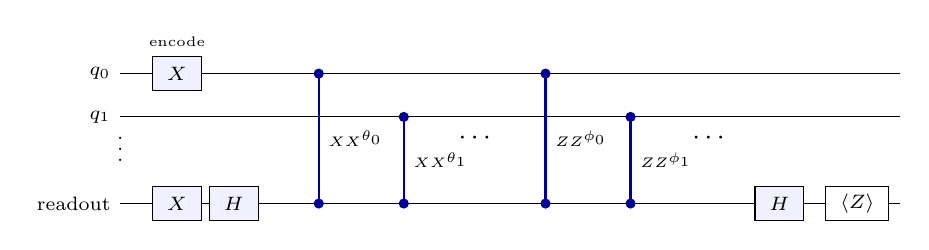
\begin{tikzpicture}[x=0.9cm,y=0.55cm,
  g/.style={draw,fill=blue!6,minimum width=0.62cm,minimum height=0.44cm,inner sep=1pt,font=\scriptsize},
  dot/.style={circle,fill=blue!60!black,inner sep=1.3pt}]
  \foreach \y/\n in {2/{$q_0$},1/{$q_1$}} \draw (0,\y) node[left,font=\scriptsize]{\n} -- (11,\y);
  \node[font=\scriptsize] at (0,0.45) {$\vdots$};
  \draw (0,-1) node[left,font=\scriptsize]{readout} -- (11,-1);
  \node[g] at (0.8,2) {$X$};
  \node[font=\tiny,above] at (0.8,2.4) {encode};
  \node[g] at (0.8,-1) {$X$}; \node[g] at (1.6,-1) {$H$};
  \foreach \x/\y/\l in {2.8/2/XX^{\theta_0},4.0/1/XX^{\theta_1},6.0/2/ZZ^{\phi_0},7.2/1/ZZ^{\phi_1}} {
    \draw[blue!60!black,thick] (\x,\y) -- (\x,-1);
    \node[dot] at (\x,\y) {}; \node[dot] at (\x,-1) {};
    \node[font=\tiny,right] at (\x,{(\y-1)/2}) {$\l$};
  }
  \node at (5.0,0.5) {$\cdots$}; \node at (8.3,0.5) {$\cdots$};
  \node[g] at (9.3,-1) {$H$};
  \node[g,fill=white,minimum width=0.8cm] at (10.4,-1) {$\langle Z\rangle$};
\end{tikzpicture}

\caption{The QNN circuit, with two of the 16 data qubits drawn. Each data qubit couples to the
readout qubit through one trainable $XX$ gate and one trainable $ZZ$ gate.}
\label{fig:circuit}
\end{figure}

\paragraph{Training.}
All models minimise the hinge loss on labels $\pm1$ with Adam \citep{kingma2014adam} (learning rate
\valMnistLr{}, batch size \valMnistBatch{}) for \valMnistEpochs{} epochs, over \valMnistSeeds{} seeds.
Quantum models are simulated exactly and differentiated with the adjoint method. We report mean
$\pm$ standard deviation over seeds. We chose the batch size and learning rate from two candidate
settings on seed 0.

\paragraph{Barren plateaus.}
Following \citet{mcclean2018barren}, each random circuit applies $R_y(\pi/4)$ to every qubit, then
layers of a uniformly random choice of $R_x$, $R_y$ or $R_z$ per qubit followed by a CZ ladder. We
estimate $\mathrm{Var}[\partial\langle Z_0Z_1\rangle/\partial\theta_0]$ over \valBpCircuits{} random
circuits and angles, sweeping \valBpMinQ--\valBpMaxQ{} qubits at \valBpFixedDepth{} layers, and
\valBpMinDepth--\valBpMaxDepth{} layers at \valBpFixedQubits{} qubits.

\paragraph{Noise.}
A single-qubit depolarizing channel with probability $p$ follows every moment of the model circuit.
Expectations average \valNoiseReps{} quantum trajectories. We run two measurements. (i) The
$4\times4$ QNNs trained above are tested under noise on \valNoiseEvalNTest{} test images (a separate
random draw from the one in Table~\ref{tab:mnist}, so the noise-free accuracies differ slightly). (ii) Models
are trained and tested with the noise present. Training through trajectories needs parameter-shift
gradients, which made 17 qubits too slow, so (ii) uses $\valNoiseSize\times\valNoiseSize$ images
(\valNoiseQubits{} qubits), \valNoiseNTrain{} training and \valNoiseNTest{} test images,
\valNoiseEpochs{} epochs, batch size \valNoiseBatch{} and learning rate \valNoiseLr{}.

\paragraph{Software and hardware.}
TensorFlow \valVerTF, TensorFlow Quantum \valVerTFQ{} and Cirq \valVerCirq, in a Linux Docker container
with 8 CPU cores on an Intel laptop, with no GPU.
